\section{Scenario 3}\label{sec:scenario3}
The purpose of this scenario is to show what can happen when the UA comes above the GS, as seen on the map in Figure \ref{fig:s3_map}. Also, the controller used in the simulation is a PD controller.

\begin{figure}[H]
	\hfill
	\subfigure[UAS Map Positioning]{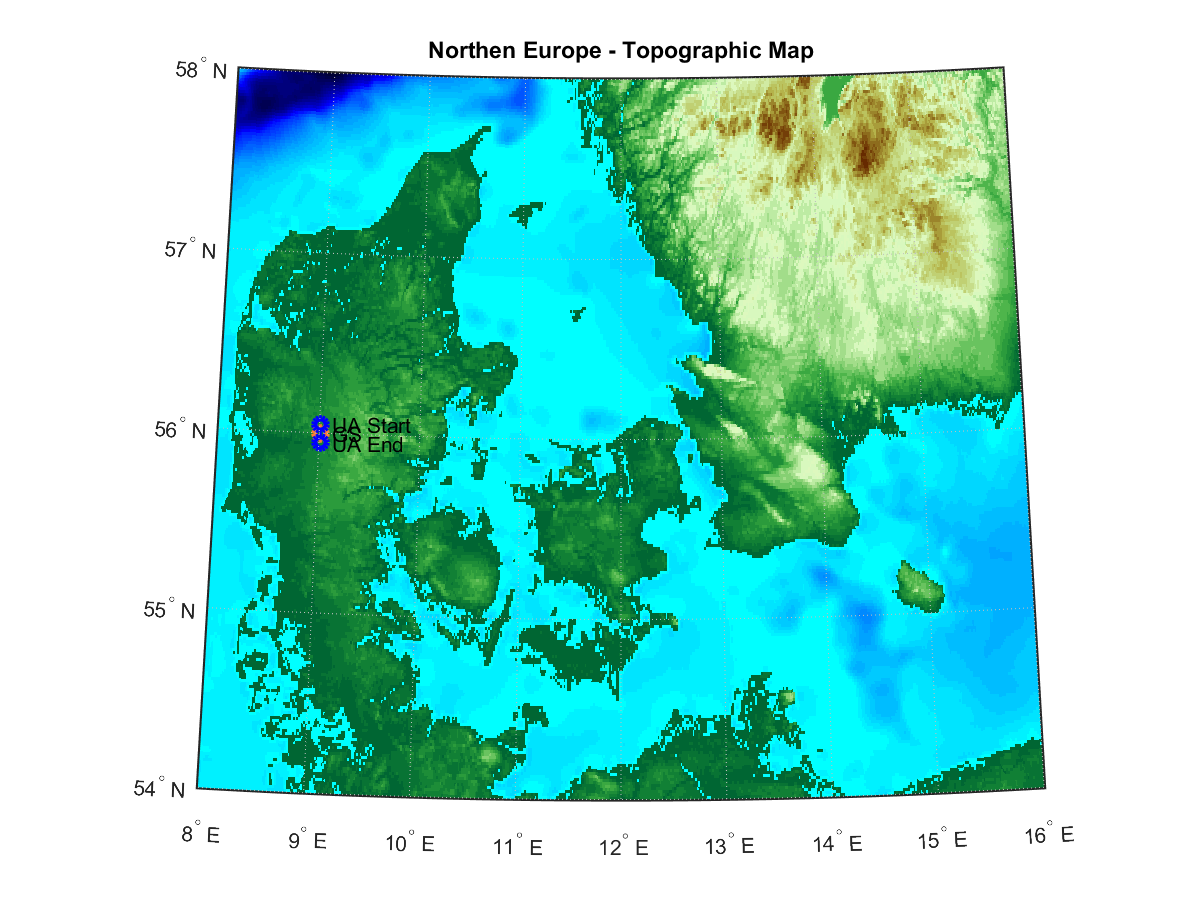
\includegraphics[scale=0.33]{figures/s3_map.png}}
	\hfill
	\subfigure[LOS and Distance]{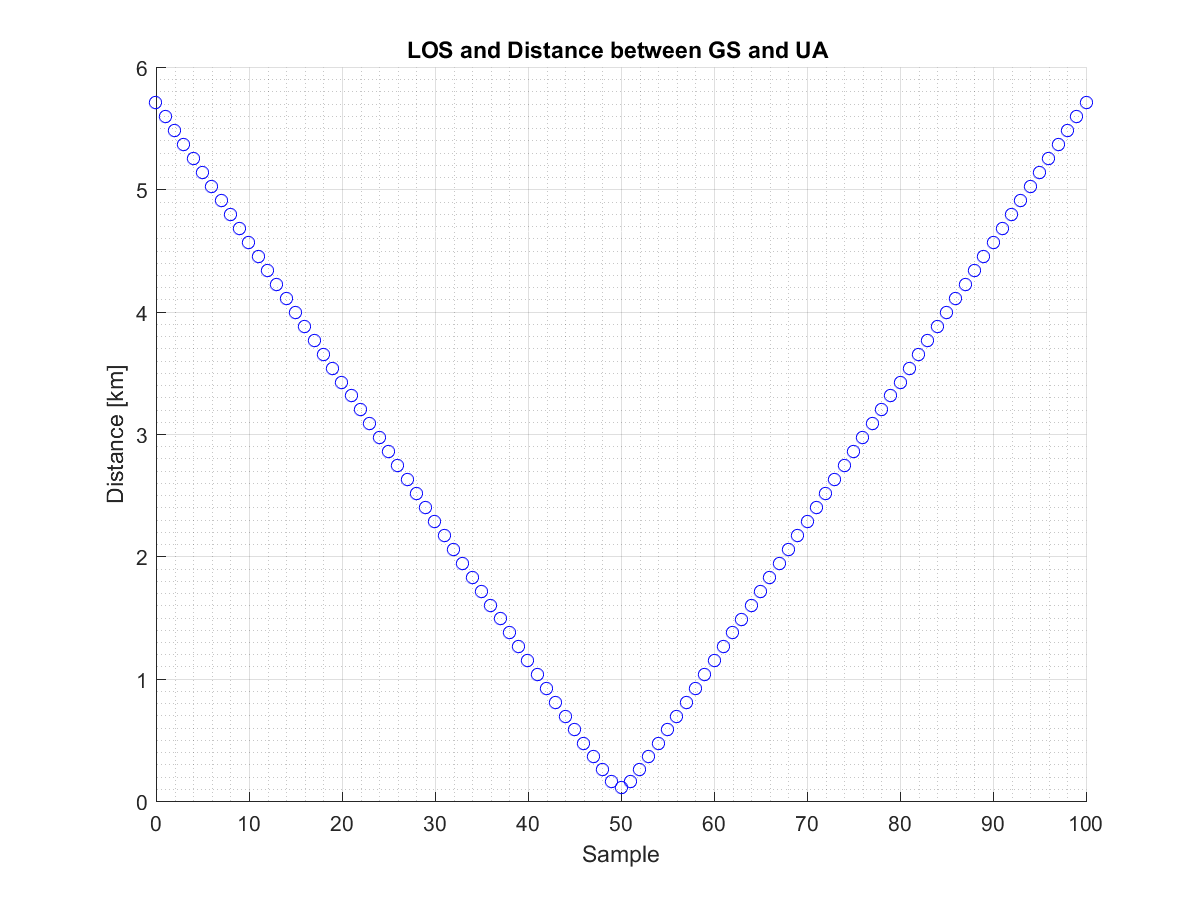
\includegraphics[scale=0.33]{figures/s3_los.png}}
	\hfill
	\caption{Mountain Scenario}
	\label{fig:s3_map}
\end{figure}

\subsection{UA}
In Figure \ref{fig:s3_ua} the angle tracking of the UA antenna can be seen.

\begin{figure}[H]
	\centering
	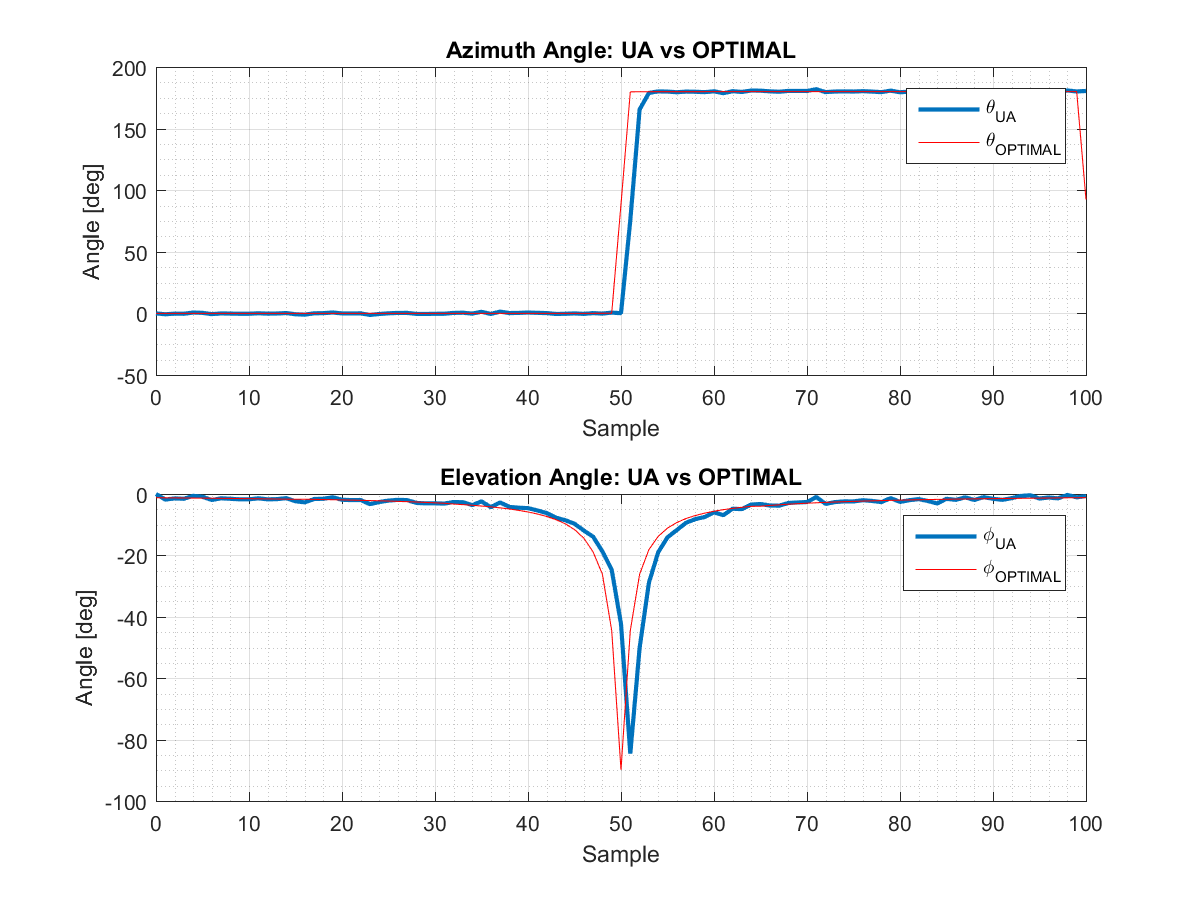
\includegraphics[scale=0.75]{figures/s3_ua.png}
	\caption{Azimuth and elevation angles of UA following the optimal angle}
	\label{fig:s3_ua}
\end{figure}

\subsection{GS}
In Figure \ref{fig:s3_gs} the angle tracking of the GS antenna can be seen.

\begin{figure}[H]
	\centering
	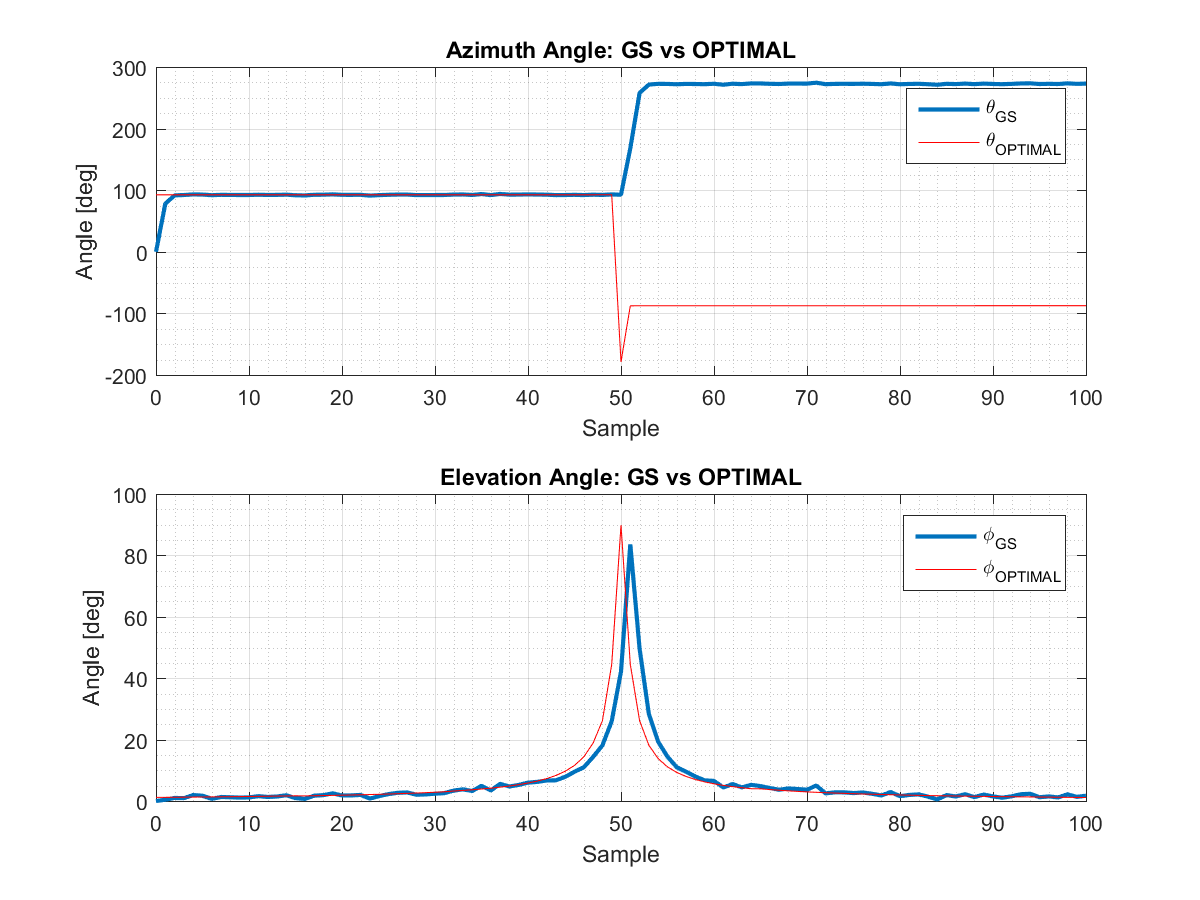
\includegraphics[scale=0.75]{figures/s3_gs.png}
	\caption{Azimuth and elevation angles of GS following the optimal angle}
	\label{fig:s3_gs}
\end{figure}

\subsection{Power}
In Figure \ref{fig:s3_power} the power at the receiver antenna of the GS antenna can be seen.

\begin{figure}[H]
	\centering
	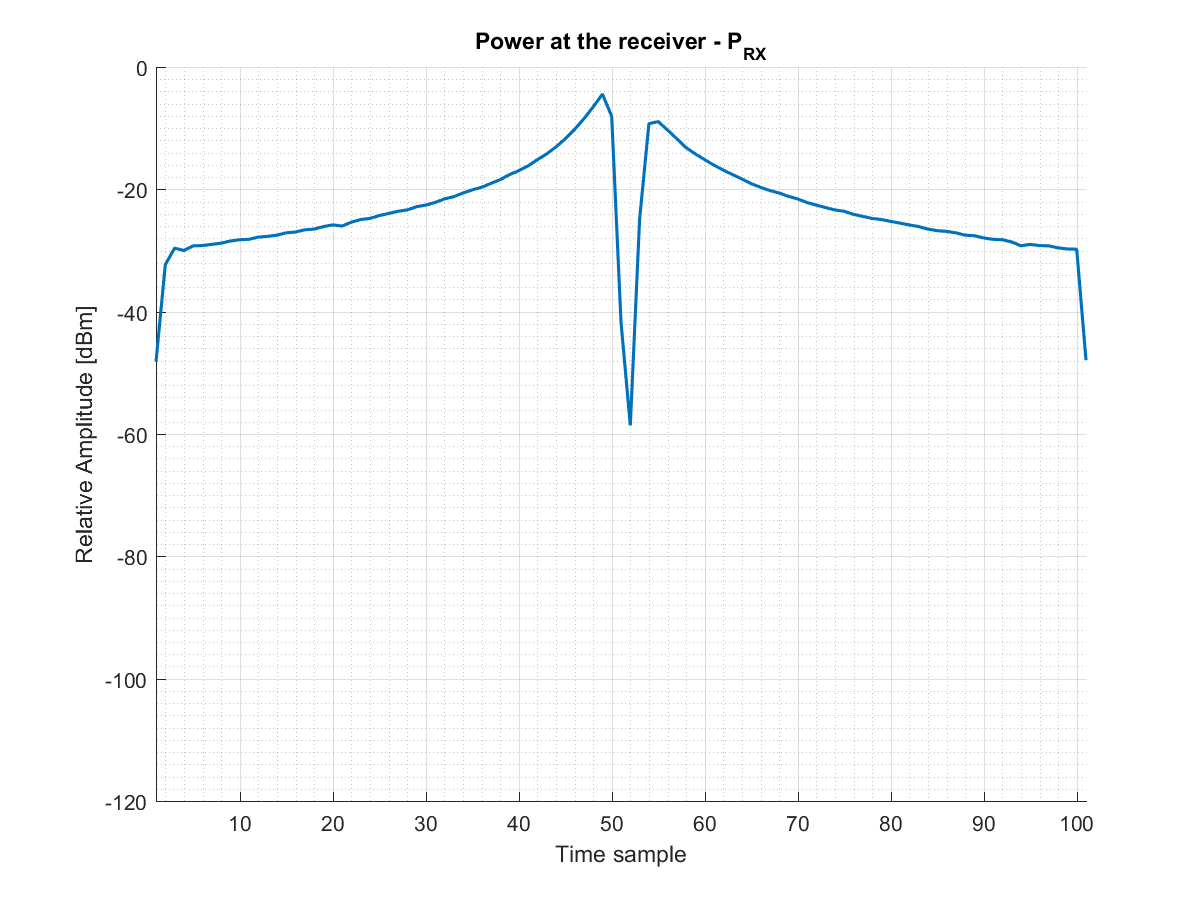
\includegraphics[scale=0.75]{figures/s3_power.png}
	\caption{Power at the receiver's antenna (GS)}
	\label{fig:s3_power}
\end{figure}